\documentclass[twoside,a4paper,11pt]{book}
\usepackage[twoside,a4paper,top=25mm,bottom=25mm,left=20mm,right=20mm]{geometry}

\usepackage{float}
%\usepackage{graphics}
\usepackage[dvips]{epsfig,rotating}
\usepackage{longtable,booktabs}
\usepackage{verbatim}
\usepackage{listings}
\usepackage[table]{xcolor}
\usepackage{forest}
 
\definecolor{codegreen}{rgb}{0,0.6,0}
\definecolor{codegray}{rgb}{0.5,0.5,0.5}
\definecolor{codepurple}{rgb}{0.58,0,0.82}
\definecolor{backcolour}{rgb}{0.95,0.95,0.92}

\lstdefinestyle{mystyle}{
    backgroundcolor=\color{backcolour},   
    commentstyle=\color{codegreen},
    keywordstyle=\color{magenta},
    numberstyle=\tiny\color{codegray},
    stringstyle=\color{codepurple},
    basicstyle=\ttfamily\footnotesize,
    breakatwhitespace=false,         
    breaklines=true,                 
    captionpos=b,                    
    keepspaces=true,                 
    numbers=left,                    
    numbersep=5pt,                  
    showspaces=false,                
    showstringspaces=false,
    showtabs=false,                  
    tabsize=2
}
 
\lstset{style=mystyle}


\usepackage{amsmath}
\usepackage{amssymb}
\usepackage{siunitx}

%\usepackage{html}

% Table Settings
\usepackage{longtable}
\usepackage{tabu}
\usepackage{multirow}
\usepackage{tabularx}
% \usepackage{makecell}
\tabulinesep=^1mm_1mm
\renewcommand{\arraystretch}{1.1}

\usepackage{caption}
\captionsetup[table]{skip=2pt}

\usepackage{todonotes}
%\usepackage{draftwatermark}

\usepackage{fancyvrb}

% Colours
\definecolor{cverbbg}{gray}{0.95}
\definecolor{cverbbd}{gray}{0.35}
\definecolor{notered}{rgb}{0.70,0.0,0.0}
\definecolor{linkred}{rgb}{0.70,0.1,0.0}

% Links
\usepackage{hyperref}
\usepackage{url}
\hypersetup{colorlinks=true, citecolor=blue, urlcolor=blue, linkcolor=linkred}
\urlstyle{same}

% Index
\usepackage{makeidx}
\makeindex

% Verbatim Box
\newenvironment{cverbatim}
 {\SaveVerbatim{cverb}}
 {\endSaveVerbatim
  \scriptsize\flushleft\addtolength{\leftskip}{5mm}
  \fboxrule=0.4pt\fboxsep=0.6em
  \fcolorbox{cverbbd}{cverbbg}{\BUseVerbatim{cverb}}%
  \endflushleft\normalsize
}

\newenvironment{ctverbatim}
 {\SaveVerbatim{ctverb}}
 {\endSaveVerbatim
  \tiny\flushleft\addtolength{\leftskip}{5mm}
  \fboxrule=0.4pt\fboxsep=0.6em
  \fcolorbox{cverbbd}{cverbbg}{\BUseVerbatim{ctverb}}%
  \endflushleft\normalsize
}

\setcounter{secnumdepth}{3}
\setcounter{tocdepth}{3}
\pagestyle{headings}
\raggedbottom

% Page Layout
%*************

\usepackage{fancyhdr}

% Plain Page Numbering
\fancypagestyle{plain}{
    \fancyhf{}
    \fancyfoot[LE,RO]{\thepage}
}

% Header style for numbered chapters
\newcommand{\defaulthead}{
    \fancyhead[LE]{\nouppercase{\scshape\leftmark}}
    \fancyhead[RO]{\nouppercase{\scshape\rightmark}}
}

% Custom heading for unnumbered chapters
\newcommand{\simplehead}[1]{
    \fancyhead[LE]{\nouppercase{\itshape #1}}
    \fancyhead[RO]{\nouppercase{\itshape #1}}
}

\pagestyle{fancy}

% Page Header
\renewcommand{\chaptermark}[1]{\markboth{\chaptername\ \thechapter: #1}{}}
\renewcommand{\sectionmark}[1]{\markright{\thesection\ #1}{}}
\renewcommand{\headrulewidth}{0pt}
\renewcommand{\footrulewidth}{0pt}

\fancyhf{}
\defaulthead
\headheight 15pt
\fancyfoot[LE,RO]{\thepage}

% Main Document
\begin{document}

\frontmatter
\pagenumbering{roman}

\pdfbookmark{Title Page}{TitlePage}
\begin{titlepage}
\begin{center}\normalsize\scshape
    European Organization for Nuclear Research \\
    CERN BE/ABP
\end{center}
\vspace*{2mm}
\begin{flushright}
    CERN/**/** \\
    Updated October 2019
\end{flushright}
\begin{center}\Huge
    \textbf{PySixDesk} \\
    \LARGE Version 1.0 \\
    \vspace*{8mm}The running Environment for SixTrack \\
    \vspace*{8mm}\textbf{User's Reference Manual}
\end{center}
\begin{center}
    X.~Lu (CSNS, CERN),
    A.~Mereghetti (CERN),
    L.~Coyle (EPFL, CERN)
\end{center}
\begin{center}\large
    \vspace*{10mm}\textbf{Abstract} \\
\end{center}
The aim of PySixDesk is to manage and control massive sixtrack simulations starting from a MADX input file. 

\vfill
\begin{center}
    Geneva, Switzerland \\
    \today
\end{center}

\end{titlepage}

\cleardoublepage

\pdfbookmark{Acknowledgements}{Acknowledgements}
\chapter*{Acknowledgement}

We would like to thank our colleagues at CERN to help us to find nasty bugs and for a thorough check of the program.

\bigskip
\begin{flushright}
    -- \textit{...}
\end{flushright}

\cleardoublepage

\pdfbookmark{Contents}{Contents}
\tableofcontents
\cleardoublepage
\pagenumbering{arabic}

% Chapters
\mainmatter

\chapter{Introduction} \label{Intro}

pySixDesk is a novel platform for managing massive simulations using sixtrack  which is a single particle tracking code widely used at CERN. It allows to set up and manage job submission, gather results and analyse them. pySixDesk comes as a python library, hence, it can be imported into a python terminal or into custom-made python scripts.

The pySixDesk package could be obtained from github repository:

\url{https://github.com/SixTrack/pysixdesk}


\paragraph{The requirements:}~

The native environment of pySixDesk is CERN's lxplus login service;The guidelines in the following will assume that this is the case.
\begin{enumerate}
    \item AFS and openAFS for disk storage;
    \item kerberos for login and user identification;
    \item htcondor, as batch service native at CERN;
    \item BOINC, as additional batch service for long-term, large simulation campaigns;
    \item sqlite, for the database monitoring the progress of jobs and storing data;
    \item mysql, the central database service used to store data;
    \item python3, as main language.
\end{enumerate}

% ================================================================================================================================ %

\paragraph{Shell set-up}~

It is recommended to use pySixDesk from the python shell. Please remember to use python3. On lxplus, python3 is available as python3 command, since the default python command uses version 2.7.5.

In order to use the library, it is essential to declare in your live python environment the path where the pysixdesk package can be found. This can be accomplished adding the path to the pysixdesk package to the PYTHONPATH environment variable (in the following, \$pysixdesk\_path is the full path to pysixdesk),eg:

\begin{lstlisting}
export PYTHON=$PYTHONPATH:$pysixdesk_path/
\end{lstlisting}

or to add it to the sys.path list, e.g:

\begin{lstlisting}[language=Python]
import sys
sys.path.append(<path_to_pysixdesk>/)
\end{lstlisting}

\section{Workflow of a study}

In pysixdesk, the program will start from a configuration file named 'config.py'. It contains all the necessary parameters needed by the jobs, such as database type, name of template file, pathes of madx and sixtrack executable, boinc spool directory, scan parameters for sixtrack and so on.

Due to the input files of an acutal sixtrack job are generated by madx, so the progress is divided into two parts. The first part is called preprocess job which will execute madx to generate input files for sixtrack, and other steps such as one-turn job for DA study, merge aperture node into fort.2 for collimation study. The second part is the sixtrack job which will execute the actual sixtrack job.

There are two scripts 'preprocess.py' and 'sixtrack.py' in the program corresponding to these two parts respectively.
\paragraph{preprocess jobs}~

The workflow of preprocess job is shown in Figure \ref{fig1}, all the studies will start from a single *.mask file. The mask file has some placeholders to generate the actual madx input files by replacing the placeholders with the given values.
\begin{lstlisting}
.....
! A Laundau octupole current 20A inj, -570A col
I_MO=%OCT;

!General switch to select collision (0/1)
ON_COLLISION:=0;
!General switch to install bb lens (0/1)
ON_BB_SWITCH:=0;
......
\end{lstlisting}

For the upper example, the user should set 'self.madx\_params['OCT'] = 0' in the config file to generate an acutal madx input file.

\begin{figure}[h]
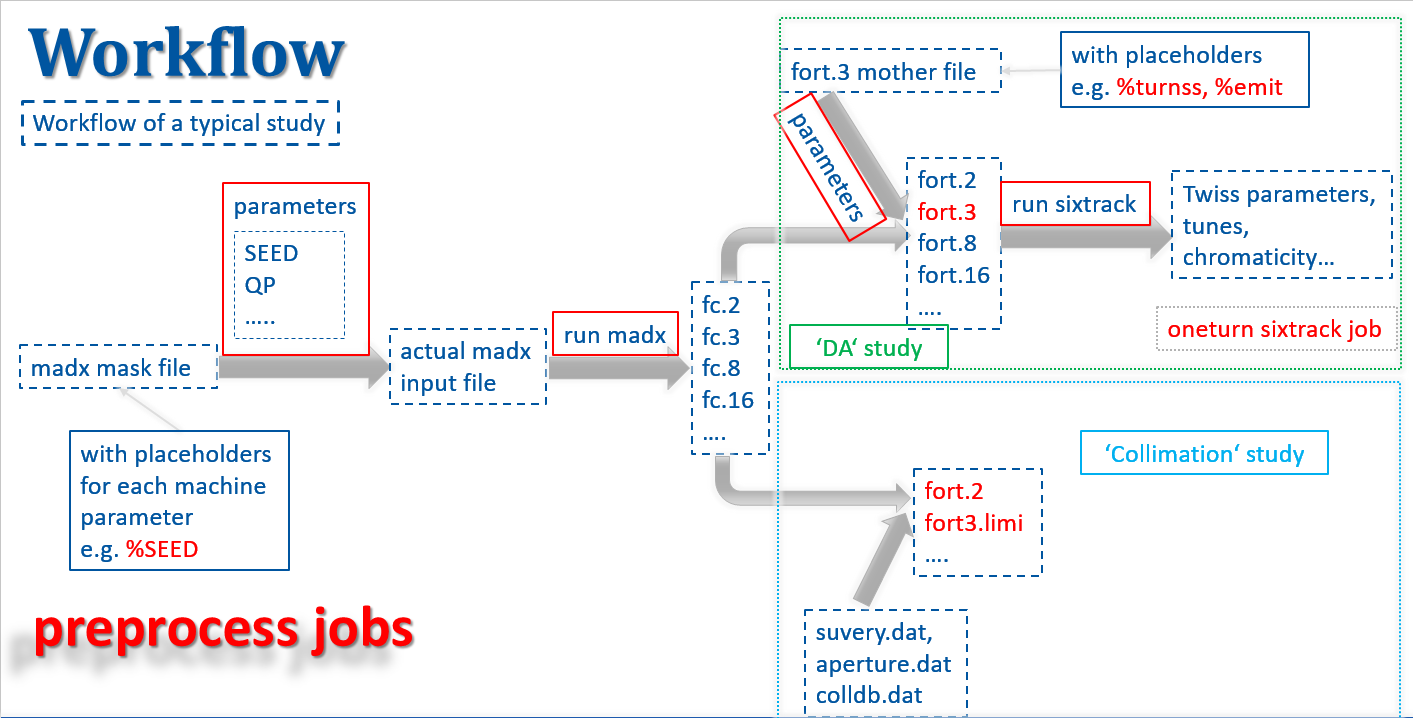
\includegraphics[width=17cm]{preprocess.png}
\caption{The workflow of preprocess job}
\label{fig1}
\centering
\end{figure}

The program will create the actual madx input file and execute madx to generate files for sixtrack jobs. In general, they will be 'fc.2', 'fc.3', 'fc.8', 'fc.16'. If the user is working on dynamic aperture (DA) study, the one-turn sixtrack job is needed to get the twiss-parameters. If the user is working on collimation study, an additional step to merge aperture model onto fort.2 is needed.

Note that the oneturn step will disappear once the new DIST block in sixtrack is done(which is ongoing), and also the additional step for merging aperture model will disappear once aperture markers and aperture offsets can be consistently generated by MADX.


\paragraph{sixtrack job}~

After the preprocess jobs are finished, the user can begin to prepare and submit sixtrack jobs. The workflow of sixtrack job is shown in Figure \ref{fig2}, the job will start from a template file 'fort.3' with some placeholders. The program will replace the placeholders with the corresponding values defined in config.py to generate the actual input file 'fort.3', the execute sixtrack to generate the required results.
\begin{figure}[h]
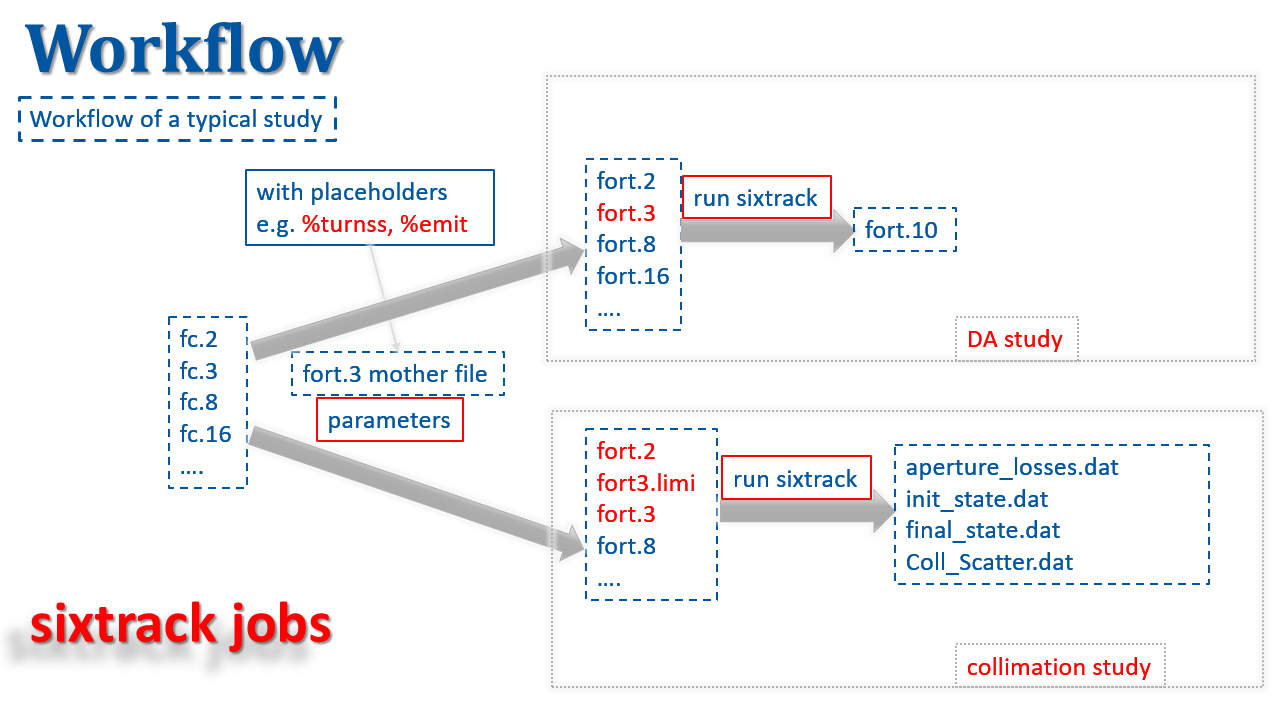
\includegraphics[width=17cm]{sixtrack.png}
\caption{The workflow of sixtrack job}
\label{fig2}
\centering
\end{figure}

The detailed command to manage these steps will introduce in the next chapter.

\section{Database}

In pySixDesk, sqlite3 and mysql are employed as the main databases to store the data. sqlite3 is the local file-based db, and mysql is the server-based db. For sqlite3 database, it will sit in your study path with an unified name \textbf{data.db}, and for mysql database, we use the DB-On-Demand server which is managed by CERN IT.
  To connect to mysql, the username, password, host, port are needed at least. For security reason, the \textbf{config.py} doesn't hold these information, the user should prepare a config file \textbf{.my.cnf} under the home directory \textbf{(\$HOME)} which contains the information, it looks like:
\begin{lstlisting}
[client]
user = test1
password = test
host = 127.0.0.1
port = 3306
\end{lstlisting}

\paragraph{Tables}~

There are several tables for a study in the database. 
\begin{lstlisting}[language=Python]
boinc_vars # for boinc variable
env # for some general valriables 
templates # template files, such as *.mask, fort.3
preprocess_wu # parameters for preprocess job
preprocess_task # records for all the preprocess tasks (each submission)
oneturn_sixtrack_wu # parameters for one-turn parameters
sixtrack_wu # parameters for sixtrack job
sixtrack_task # records for all the sixtrack task (each submission)

oneturn_sixtrack_results # results of one turn sixtrack jobs
six_results # results of actual sixtrack jobs
#some general info of the tracking
init_state
final_state
aperture_losses
#results of collimation study
collimation_losses
\end{lstlisting}
The detailed description of the tables can be found in \url{https://github.com/SixTrack/pysixdesk/blob/master/doc/Table.md}

\paragraph{Special features}~

There are also some special features in pysixdesk:
\begin{enumerate}
\item submit from local computer. Due to HTCondor have the spooling ability, so the user can submit jobs from a local computer. To use this feature, the user should setup kerberos and HTCondor on a local computer at first. Here is a sample instruction:
\url{https://twiki.cern.ch/twiki/bin/view/ABPComputing/LxbatchHTCondor}. 

Note that the user should submit jobs with '-spool' option from a local computer.

\item group the jobs. pysixdesk could group the jobs by the given parameter. e.g. group by amplitude, then each group will have all scanned values of amplitude but same values of other parameters. And a group will be submitted to one HTCondor node.

\item prolong tracking. pysixdesk could prolong the tracking with checkpoint/restart feature. There are three flag in config.py to switch this feature, 'self.checkpoint\_restart = False', 'self.first\_turn=1', 'self.last\_turn=100'. If checkpoint\_restart is set to True, the program will find the checkpoint files (if exist) and prolong the complete job. 

Note that the user should make sure the sixtrack executable in use is compiled with the CR option.
\end{enumerate}

\paragraph{Tests}~

Below is a scalability test result for different databases. The test condition: 300 preprocess jobs, 30000 sixtrackjobs. All operations were done on CERN lxplus and all jobs were submitted to HTCondor.
\begin{table}[h]
    \caption{Scalability tests for these two databases.}
    \label{T-ExtRou}
    \centering
    \renewcommand{\arraystretch}{1.5}
    \begin{tabular}{|l|l|l|}
        \hline
        \rowcolor{blue!30}
        \textbf{Action/DB} & \textbf{Sqlite3} & \textbf{Mysql} \\
        \hline
        \texttt{setup DB}  & 5s & 11s \\
        \hline
        \texttt{prepare preprocess}  & 1s & 1s \\
        \hline
        \texttt{submit}   & 6s    & 27s \\
        \hline
        \texttt{collection}   & 120s   & - \\
        \hline
        \texttt{prepare sixtrack}  & 240s & 128s \\
        \hline
        \texttt{submit}   & 435s    & 294s \\
        \hline
        \texttt{collection}   & ~3h   & - \\
        \hline
    \end{tabular}
\end{table}

Where '-' represent no need.
Note that if the user select mysql and submit jobs to BOINC, the collection process is still needed. For the moment, the volunteer computers can't access to the mysql server directly.

%\subsection{Command Line Arguments} \label{sec:cmdarg}
%
%SixTrack does not require any command line arguments, but can optionally take the file name for the main input file as well as the geometry file as the first and second argument, respectively.
%See also Sections~\ref{InFiles} and~\ref{ProVer}.
%
%\bigskip
%\noindent In addition, SixTrack can echo the version number and exit with the following flags:
%\begin{itemize}
%    \item[\texttt{-v}] Echo program name and version as a single line, and exit.
%    \item[\texttt{-V}] Echo program name, version, release date, and git hash on four lines, and exit.
%    \item[\texttt{-nv}] Echo the numerical version as an integer, and exit,
%\end{itemize}

\cleardoublepage

\chapter{Detailed Guide}

\section{Step-by-Step Guide}

This section will introduce the detailed steps and logics to setup a workspace and an actual study.

\subsection{set up the worksapce}
After importing all the necessary modules from pysixdesk, a workspace could be setup by the following command:
\begin{lstlisting}[language=Python]
myWS = WorkSpace('./myWS')
\end{lstlisting}
where \textbf{'./myWS'} is the workspace name, this step will create a new folder with the following tree structure:

\begin{forest}
  for tree={
    font=\ttfamily,
    grow'=0,
    child anchor=west,
    parent anchor=south,
    anchor=west,
    calign=first,
    edge path={
      \noexpand\path [draw, \forestoption{edge}]
      (!u.south west) +(7.5pt,0) |- node[fill,inner sep=1.25pt] {} (.child anchor)\forestoption{edge label};
    },
    before typesetting nodes={
      if n=1
        {insert before={[,phantom]}}
        {}
    },
    fit=band,
    before computing xy={l=15pt},
  }
[myWS/
  [studies/
  ]
  [templates/
    [hl10.mask]
    [fort.3]
    [config.py]
    [htcondor\_run.sub]
    [CollDB.data]
  ]
]
\end{forest}

The studies folder contains different studies. A new study folder will be added when the user initialize a study.

All the files under templates folder were copied from the templates folder in pysixdesk program by default. The user can use different templates as needed by assigning the argument 'templates' to a custom path:
\begin{lstlisting}[language=Python]
myWS = WorkSpace('./myWS', templates = <your path>)
\end{lstlisting}
The program will copy templates from $<$your path$>$, so in $<$your path$>$ there should have 'config.py', 'mask file', 'fort.3' and 'htcondor\_run.sub' at least.

\subsection{set up a study}
After setting up the workspace, a study could be initialized by the following command:

\begin{lstlisting}[language=Python]
myWS.init_study('myStudy')
\end{lstlisting}
This action will create a new study folder under 'studies' folder with the following tree structure:

\begin{forest}
  for tree={
    font=\ttfamily,
    grow'=0,
    child anchor=west,
    parent anchor=south,
    anchor=west,
    calign=first,
    edge path={
      \noexpand\path [draw, \forestoption{edge}]
      (!u.south west) +(7.5pt,0) |- node[fill,inner sep=1.25pt] {} (.child anchor)\forestoption{edge label};
    },
    before typesetting nodes={
      if n=1
        {insert before={[,phantom]}}
        {}
    },
    fit=band,
    before computing xy={l=15pt},
  }
  [studies/
    [myStudy/
      [config.py]
      [hl10.mask]
      [fort.3]
      [htcondor\_run.sub]
      [CollDB.data]
      [preprocess\_input/]
      [preprocess\_output/]
      [sixtrack\_input/]
      [sixtrack\_output/]
    ]
  ]
\end{forest}

Note that the template files under myStudy folder were copied from the templates folder in workspace (myWS). And similarly the user can set up a study with custom template files:
\begin{lstlisting}[language=Python]
myWS.init_study('myStudy', templates=<your path>)
\end{lstlisting}

The preprocess\_input (sixtrack\_input) folder holds all the input information for preprocess (sixtrack) jobs, and preprocess\_output (sixtrack\_output) holds the results of preprocess (sixtrack) jobs.

\subsection{Config parameters}
After initilizing a study, the user should edit the 'config.py' to prepare the parameters.
The editable parameters are shown as below:
\begin{lstlisting}[language=Python]
self.paths['madx_exe']  # the path of madx executable
self.paths['sixtrack_exe'] # the path of sixtrack executable
self.paths['boinc_spool'] # the path of boinc spool
self.oneturn = True # switch for one turn sixtrack job
self.collimation = False # switch for preprocess job for collimation study (merge aperture marker into fort.2, generate fort3.limi file)

self.checkpoint_restart = False # flag for CR feature
self.first_turn = 1 # the first turn when sixtrack job continue with checkpoint file
self.last_turn = 100 # the last turn of the sixtrack tracking

self.db_info['db_type'] = 'sql' # database type 'sql' or 'mysql'
self.max_submitjob = 15000 # the maximum number of jobs to submit per cluster id
\end{lstlisting}

\begin{lstlisting}[language=Python]
#The keys are the names of madx output files, the values are the names of the input files needed by sixtrack. Due to they have the different naming covention, so there is an additional step to change the names of the files based on key-value map.
self.madx_output = {
     'fc.2': 'fort.2',
     'fc.3': 'fort.3.mad',
     'fc.3.aux': 'fort.3.aux',
     'fc.8': 'fort.8',
     'fc.16': 'fort.16',
     'fc.34': 'fort.34'}
self.madx_input['mask_file'] = 'hl10.mask'
self.madx_params = {} # The parameters for madx
#e.g.
self.madx_params['SEED'] = [1,2,3]
self.madx_params['IOCT'] = [100, 200]
self.madx_params['QP'] = [1,2,3]
.....
#Every placeholder in mask file should be found in self.madx_params dict.
\end{lstlisting}

\begin{lstlisting}[language=Python]
self.oneturn_sixtrack_input['fort_file'] = 'fort.3'
self.oneturn_sixtrack_params = {}
\end{lstlisting}

\begin{lstlisting}[language=Python]
#preprocess_output will add 'oneturnresult' automatically.
self.preprocess_output = dict{self.madx_output}
\end{lstlisting}

\begin{lstlisting}[language=Python]
self.sixtrack_input['fort_file'] = 'fort.3'
self.sixtrack_params = {} # parameters for sixtrack
#e.g.
self.sixtrack_params['amp'] = [(8,10), (10,12)]
self.sixtrack_params['kang'] = [1,2,3,4]
self.sixtrack_params['turnss'] = 100
self.sixtrack_params['nss'] = 1
self.sixtrack_params['e0'] = 7000000
......
# Every placeholder in template 'fort.3' should be found in self.sixtrack_params dict. 

self.sixtrack_input['input'] = dict(self.preprocess_output)
#The outputs of preprocess job will be the inputs for sixtrack job
self.sixtrack_input['additional_input'] = [] # additional input files needed by sixtrack jobs if any
\end{lstlisting}

For preprocess job for collimation study:
\begin{lstlisting}[language=Python]
self.collimation_input = {'aperture':'allapert.b1', 'survey':'SurveyWithCrossing_XP_lowb.dat'}
\end{lstlisting}

\begin{lstlisting}[language=Python]
# some other general parameters
self.env['emit'] = 3.75
self.env['gamma'] = 7460.5
self.env['kmax'] = 5
\end{lstlisting}

Settings of boinc:
\begin{lstlisting}[language=Python]
self.paths['boinc_spool'] = '/afs/cern.ch/work/b/boinc/boinc/'
self.boinc_vars['workunitName'] = 'pysixdesk'
self.boinc_vars['fpopsEstimate'] = 30 * 2 * 10e5 / 2 * 10e6 * 6
self.boinc_vars['fpopsBound'] = self.boinc_vars['fpopsEstimate'] * 1000
self.boinc_vars['memBound'] = 100000000
self.boinc_vars['diskBound'] = 200000000
self.boinc_vars['delayBound'] = 2400000
self.boinc_vars['redundancy'] = 2
self.boinc_vars['copies'] = 2
self.boinc_vars['errors'] = 5
self.boinc_vars['numIssues'] = 5
self.boinc_vars['resultsWithoutConcensus'] = 3
self.boinc_vars['appName'] = 'sixtrack'
self.boinc_vars['appVer'] = 50205
\end{lstlisting}

\begin{lstlisting}[language=Python]
# Select the cluster to submit jobs, HTCondor in default
self.cluster_class = submission.HTCondor 
\end{lstlisting}
And a custom cluster could be used to submit jobs. In order to use it, please make sure that the file containing the custom cluster class which extends from submission.Cluster in the path PYTHONPATH. Then just assign the cluster\_class attribute in config.py to the desired class:
\begin{lstlisting}[language=Python]
 import cluster
 ...
 def __init__(self, name='study', location=os.getcwd()):
     super(MyStudy, self).__init__(name, location)
     self.cluster_class = cluster.custom
\end{lstlisting}

\subsection{Load study}\label{loadstudy}
After the user prepare all the necessary , a study object could be loaded with the command:

\begin{lstlisting}[language=Python]
mystudy = myWS.load_study('myStudy')
\end{lstlisting}
By defaults, the program will find the configuration file 'config.py' under study path to create the study object with the default class name 'MyStudy'. But, it is also possible to create the study object with a custom configuration file and a different class name:

\begin{lstlisting}[language=Python]
mystudy = myWS.load_study('myStudy', module_path=<config file path>, class_name=custom_name)
\end{lstlisting}

During the process of creating study object, a database will be set up and the necessary directories and files will aslo be created. The concerned steps could be found in the class method 'customize'.

\subsection{Update database}
In section \ref{loadstudy}, a study object was obtained from the load\_study method. Now the user can update the DB with the given parameters:

\begin{lstlisting}[language=Python]
mystudy.update_db()
\end{lstlisting}

For the db table 'templates', 'boinc\_vars' and 'env', the program will update  the new values (overide old values) from the configuration file whenever the user call the update\_db method. And for the table 'preprocess\_wu', 'sixtrack\_wu', the program will check the parameter changes at first to avoid duplicate records and create new lines to insert the new values. 

\subsection{Prepare input files}
Before submitting jobs to batch-system, the user should prepare the necessary input files at first, such as 'htcondor\_run.sub', 'job\_id.list', 'sub.db'(for sqlite3). This can be done issuing the following command: 

\begin{lstlisting}[language=Python]
mystudy.prepare_preprocess_input()
\end{lstlisting}

This action will query all the incomplete jobs from db and write the corresponding task\_ids into job\_id.list. If the user use sqlite3 as the db, a small local db 'sub.db' will also be formed to store the necessary information needed by the jobs, this db file will be submitted to HTCondor together with the jobs.

If by any chance the jobs are removed or disappear, e.g. the user realizes wrong paratemeters are set after submission and remove all the submitted jobs via command 'condor\_rm'. The user can resubmit the jobs by the following command:
\begin{lstlisting}[language=Python]
mystudy.prepare_preprocess_input(resubmit=True)
\end{lstlisting}
This action will submit again all jobs.

For sixtrack jobs, the command is:

\begin{lstlisting}[language=Python]
mystudy.prepare_sixtrack_input()
or
mystudy.prepare_sixtrack_input(resubmit=True)
\end{lstlisting}
Sixtrack jobs can be submitted to Boinc with the following command:
\begin{lstlisting}[language=Python]
mystudy.prepare_sixtrack_input(boinc=True)
\end{lstlisting}
Please note that the jobs will be anyway submitted to HTCondor at first, and executed with a few turns to check correctness of the configuration and survival of particles within the very first turns automatically. If the job pass the test, it will be submitted to Boinc.

Another special feature of sixtrack job is that the jobs could be grouped based on a specified parameter:
\begin{lstlisting}[language=Python]
mystudy.prepare_sixtrack_input(groupby='amp')
\end{lstlisting}
This action will group the jobs wrt amplitude, and submit the groups to HTCondor which means one condor node will hold a group of jobs.

\subparagraph{pre-calculation}~

For the DA studies, there are some preliminary calculations are performed  before submitting the actual jobs, the namely calculations are defined in 'config.py' file and can be modified at user's will:
\begin{lstlisting}[language=Python]
def pre_calc(self, paramdict, pre_id):
    '''Further calculations for the specified parameters'''
    # The angle should be calculated before amplitude
    keys = list(paramdict.keys())
    status = []
    status.append(self.formulas('kang', 'angle', paramdict, pre_id))
    status.append(self.formulas('amp', ['ax0s', 'ax1s'], paramdict, pre_id))
    param_keys = list(paramdict.keys())
    [paramdict.pop(key) for key in param_keys if key not in keys]
    return all(status)

def formulas(self, source, dest, paramdict, pre_id):
    '''The formulas for the further calculations,
    this function should be customized by the user!
    @source The source parameter name
    @dest  The destination parameter name
    @paramdict The parameter dictionary, the source parameter in the dict
    will be replaced by destination parameter after calculation
    @pre_id The identified preprocess job id
    @return The status'''
\end{lstlisting}

\subsection{Submission}
If preparation of input files is succeeded, the user could find 'htcondor\_run.sub', 'job\_id.list', 'input.ini' and 'sub.db'(only for sqlite3) under preprocess\_input (for MADX/one-turn jobs) or sixtrack\_input (for actual sixtrack jobs) folder, then the user could submit the prepared jobs with the following command:
\begin{lstlisting}[language=Python]
mystudy.submit(0, 5) #0 stand for preprocess job, 5 is the maximum number of trials
or
mystudy.submit(1, 5) # 1 stand for sixtrack job
\end{lstlisting}
This action will submit the preprocess or sixtrack jobs to HTCondor.

Note: HTCondor has a limitation, the maximum number of jobs presently set of 15000 for one cluser Id. If the total number of jobs exceeds this limitation, the submission will fail. There is an argument 'max\_jobsubmit' in config file to control the maximum job number of one submission. If the total number of jobs is larger than max\_jobsubmit, the program will split all the jobs in several clusers.

\subsection{Collection}
For sqlite3 DB, the user can collect the results with the following command:
\begin{lstlisting}[language=Python]
mystudy.collect_result(0)
or
mystudy.collect_result(1)
\end{lstlisting}

This action will look through the preprocess\_output (for preprocess jobs) or sixtrack\_output (for actual sixtrack jobs) folder to get the results downloaded from HTCondor. In general, the subfolder name is the task\_id or grouped task\_ids.
Before looking through the result folder, the program will query the job status (condor\_q) firstly to check which jobs are not finished yet.

And due to the program could submit jobs to HTCondor from a local computer with 'spool' option. 
\begin{lstlisting}[language=Python]
mystudy.submit(1, '-spool')
\end{lstlisting}
So the program will also try to download results from HTCondor spool directory after checking the job status.
\begin{lstlisting}[language=Python]
unfin = cluster.check_running(studypath)#clusterId.processId
......
cluster.download_from_spool(studypath)
\end{lstlisting}

If the user submit jobs to boinc, results can be downloaded from the boinc spool directory with the following codes:
\begin{lstlisting}[language=Python]
if ('boinc' in cf['info'].keys()) and cf['info']['boinc']:
    content = "Downloading results from boinc spool!"
    logger.info(content)
    task_ids = download_from_boinc(info_sec)
\end{lstlisting}
The results from boinc will be copied to corresponding folders under sixtrack\_output directory, then be parsed and pushed to db.


%\subsection{Command Line Arguments} \label{sec:cmdarg}
%
%SixTrack does not require any command line arguments, but can optionally take the file name for the main input file as well as the geometry file as the first and second argument, respectively.
%See also Sections~\ref{InFiles} and~\ref{ProVer}.
%
%\bigskip
%\noindent In addition, SixTrack can echo the version number and exit with the following flags:
%\begin{itemize}
%    \item[\texttt{-v}] Echo program name and version as a single line, and exit.
%    \item[\texttt{-V}] Echo program name, version, release date, and git hash on four lines, and exit.
%    \item[\texttt{-nv}] Echo the numerical version as an integer, and exit,
%\end{itemize}

\cleardoublepage

\providecommand{\tightlist}{%
  \setlength{\itemsep}{0pt}\setlength{\parskip}{0pt}}

\hypertarget{python-module-index}{%
\section{Python Module Index}\label{python-module-index}}

%\protect\hyperlink{cap-p}{\textbf{p}}

\begin{longtable}[]{@{}lll@{}}
& ~ &\tabularnewline
& \textbf{p} &\tabularnewline
\href{pysixdesk.lib.html\#module-pysixdesk.lib}{\texttt{pysixdesk.lib}}
& \emph{}\tabularnewline
& ~~~
\href{pysixdesk.lib.html\#module-pysixdesk.lib.configbash}{\texttt{pysixdesk.lib.configbash}}
& \emph{}\tabularnewline
& ~~~
\href{pysixdesk.lib.html\#module-pysixdesk.lib.constants}{\texttt{pysixdesk.lib.constants}}
& \emph{}\tabularnewline
& ~~~
\href{pysixdesk.lib.html\#module-pysixdesk.lib.dbadaptor}{\texttt{pysixdesk.lib.dbadaptor}}
& \emph{}\tabularnewline
& ~~~
\href{pysixdesk.lib.html\#module-pysixdesk.lib.dbtypedict}{\texttt{pysixdesk.lib.dbtypedict}}
& \emph{}\tabularnewline
& ~~~
\href{pysixdesk.lib.html\#module-pysixdesk.lib.fort2_tools}{\texttt{pysixdesk.lib.fort2\_tools}}
& \emph{}\tabularnewline
& ~~~
\href{pysixdesk.lib.html\#module-pysixdesk.lib.gather}{\texttt{pysixdesk.lib.gather}}
& \emph{}\tabularnewline
& ~~~
\href{pysixdesk.lib.html\#module-pysixdesk.lib.generate_fort2}{\texttt{pysixdesk.lib.generate\_fort2}}
& \emph{}\tabularnewline
& ~~~
\href{pysixdesk.lib.html\#module-pysixdesk.lib.machineparams}{\texttt{pysixdesk.lib.machineparams}}
& \emph{}\tabularnewline
& ~~~
\href{pysixdesk.lib.html\#module-pysixdesk.lib.preprocess}{\texttt{pysixdesk.lib.preprocess}}
& \emph{}\tabularnewline
& ~~~
\href{pysixdesk.lib.html\#module-pysixdesk.lib.pysixdb}{\texttt{pysixdesk.lib.pysixdb}}
& \emph{}\tabularnewline
& ~~~
\href{pysixdesk.lib.html\#module-pysixdesk.lib.resultparser}{\texttt{pysixdesk.lib.resultparser}}
& \emph{}\tabularnewline
& ~~~
\href{pysixdesk.lib.html\#module-pysixdesk.lib.sixtrack}{\texttt{pysixdesk.lib.sixtrack}}
& \emph{}\tabularnewline
& ~~~
\href{pysixdesk.lib.html\#module-pysixdesk.lib.study}{\texttt{pysixdesk.lib.study}}
& \emph{}\tabularnewline
& ~~~
\href{pysixdesk.lib.html\#module-pysixdesk.lib.submission}{\texttt{pysixdesk.lib.submission}}
& \emph{}\tabularnewline
& ~~~
\href{pysixdesk.lib.html\#module-pysixdesk.lib.twiss_tools}{\texttt{pysixdesk.lib.twiss\_tools}}
& \emph{}\tabularnewline
& ~~~
\href{pysixdesk.lib.html\#module-pysixdesk.lib.utils}{\texttt{pysixdesk.lib.utils}}
& \emph{}\tabularnewline
& ~~~
\href{pysixdesk.lib.html\#module-pysixdesk.lib.workspace}{\texttt{pysixdesk.lib.workspace}}
& \emph{}\tabularnewline
\bottomrule
\end{longtable}

%\hypertarget{pysixdesk}{%
%\section{\texorpdfstring{\href{index.html}{pysixdesk}}{pysixdesk}}\label{pysixdesk}}
%
%\hypertarget{navigation}{%
%\subsubsection{Navigation}\label{navigation}}
%
%\hypertarget{related-topics}{%
%\subsubsection{Related Topics}\label{related-topics}}
%
%\begin{itemize}
%\tightlist
%\item
%  \href{index.html}{Documentation overview}
%\end{itemize}
%
%\hypertarget{searchbox}{}
%\hypertarget{quick-search}{%
%\subsubsection{Quick search}\label{quick-search}}
%
%©2019, Xiaohan Lu, Alession Mereghetti. \textbar{} Powered by
%\href{http://sphinx-doc.org/}{Sphinx 1.7.9} \&
%\href{https://github.com/bitprophet/alabaster}{Alabaster 0.7.8}
%
%\end{document}

\cleardoublepage
%\input{chGeneralUse}
%\cleardoublepage

%\appendix
%\pdfbookmark{Appendix}{Appendix}
%\phantomsection
%\part*{Appendix}
%
%\renewcommand{\chaptername}{Appendix}
% \input{apxKeywords}
% \cleardoublepage
%\input{apxDefaults}
%\cleardoublepage
%\input{apxInputOutput}
%\cleardoublepage
%\input{apxDataStructure}
%\cleardoublepage
% \input{apxExamples}
% \cleardoublepage

\backmatter
\begin{thebibliography}{99}
    %
    \bibitem{DALIE}
       Test.
    %
    \addcontentsline{toc}{chapter}{Bibliography}
\end{thebibliography}

\cleardoublepage

\pdfbookmark{Keyword Index}{Index}
\printindex
\cleardoublepage

%\pdfbookmark{List of Tables}{List of Tables}
%\listoftables
%\cleardoublepage

\end{document}
